\startchapter{Results and Evaluation}
\label{chapter:eval}

This chapter presents results using the experimental set-up given in the previous chapter (Chapter \ref{chapter:Exp}). We evaluate the learning algorithm with respect to the omniscient policy. Before evaluation we need to first find optimal values for hyper-parameters $\alpha$ (Section \ref{chap6:alpha}) and confidence threshold $C$ (Section \ref{chap6:threshold}). We then proceed to use these optimal values to evaluate the learning algorithm with and without the skip feature. (Section \ref{chap6:la}). 

% Up until now, we did not penalize content items which gave no rewards. However, in section \ref{chap6:pr} we penalize such content items.

\section{Confidence Bound $\alpha$ \label{chap6:alpha}}

Finding an optimal value for $\alpha$ is important to learn faster as it scales the confidence bound of each content item. An optimal value would find the right balance between exploration and exploitation. A higher value of $\alpha$ would imply the learning algorithm takes more rounds exploring which can lead to sub-optimal results. \par

This parameter is configured for the learning algorithm and not the omniscient policy. We empirically evaluated an optimal value for $\alpha$ using course 1 (Section: \ref{chap5:courses}). The graph (Figure \ref{chap6:rpr_alpha}) shows the cumulative reward for different values of $\alpha$. \par

% \begin{figure}[H]
%     \centering
%     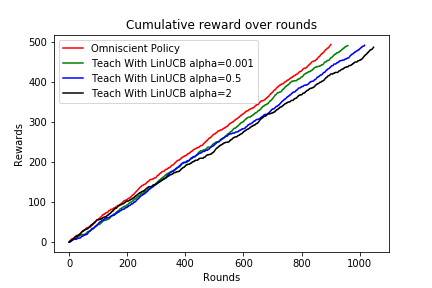
\includegraphics[scale=1.0]{Figures/optimal_alpha.png}
%     \caption{Cumulative reward per $\alpha$.}
%     \label{alpha}
% \end{figure}

\begin{figure}[H]
    \centering
    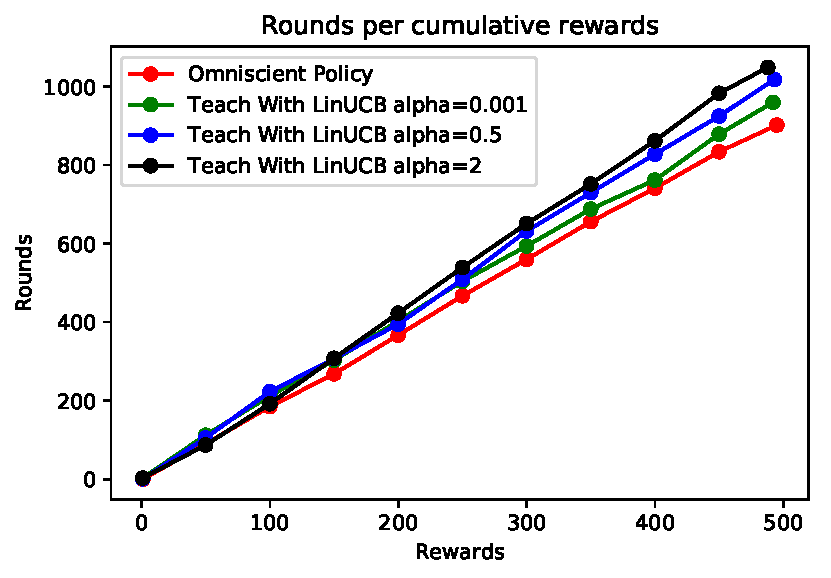
\includegraphics[scale=1.0]{Figures/rounds_per_reward_for_alpha.pdf}
    \caption{Rounds per cumulative reward for $\alpha$.}
    \label{chap6:rpr_alpha}
\end{figure}

The graph (Figure \ref{chap6:rpr_alpha}) compares the omniscient policy with the learning algorithm for different values of $\alpha$. It shows that the learning algorithm \textbf{took 960 rounds to maximize reward when} $\mathbf{\alpha = 0.001}$ compared to 1018 rounds required by $\alpha = 0.5$ and 1049 rounds required by $\alpha = 2$. On repeated run of the same experiment, we found that a value of $\alpha$ between 0 to 0.5 gives better results.\textbf{We would be using $\alpha = 0.001$ to evaluate the learning algorithm.} \par

The graph (Figure \ref{chap6:rprr_alpha}) presents a different view of the above graph. It shows the number of rounds to reward ratio at different intervals for different values of $\alpha$ and compares it to the omniscient policy. It clearly shows that $\alpha = 0.001$ required the fewest rounds to maximize reward. 

\begin{figure}[H]
	\centering
    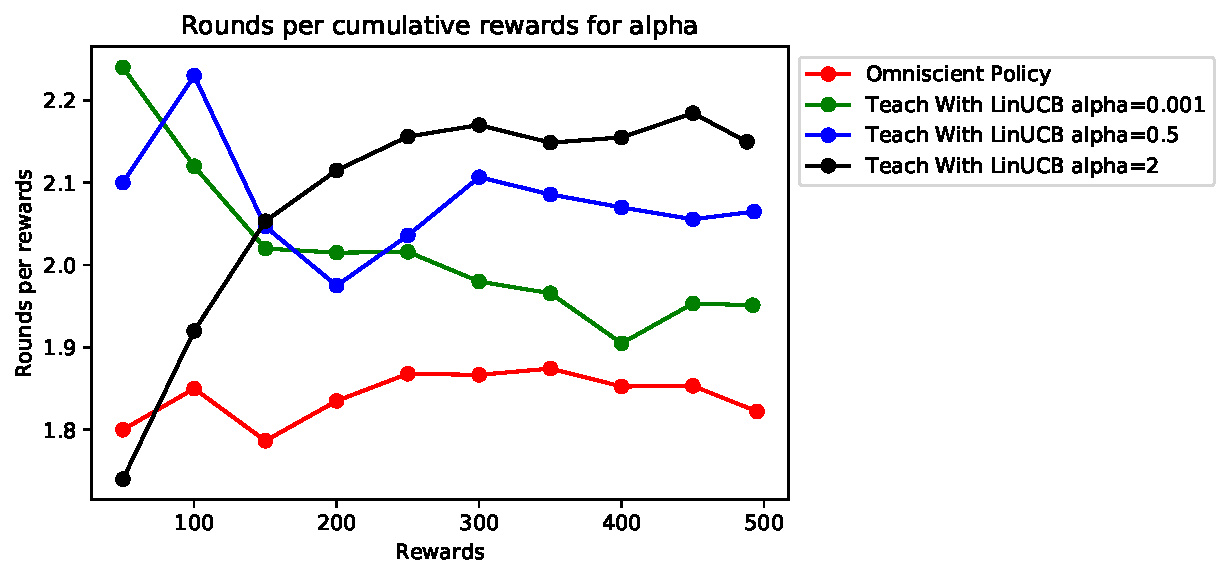
\includegraphics[scale=0.85]{Figures/rounds_per_reward_ratio_for_alpha.pdf}
    \caption{Rounds per cumulative reward ratio for $\alpha$.}
    \label{chap6:rprr_alpha}
\end{figure}

% The graph \ref{chap6:rpr_omni} presents a different view of the above graph. It shows the number of extra rounds required for different value's of $\alpha$ compared to the omniscient policy. It clearly shows that $\alpha = 0.001$ required the fewest rounds to maximize reward. 

% \begin{figure}[H]
%     \centering
%     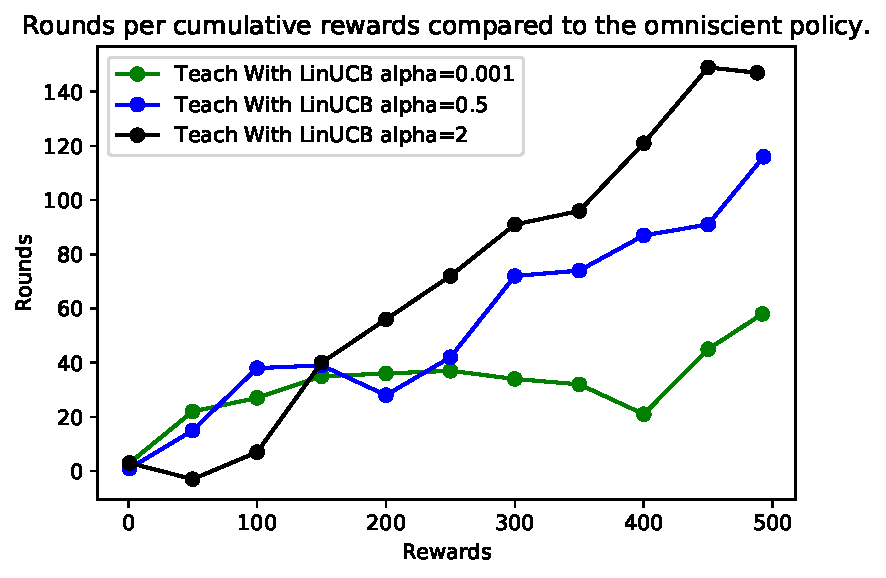
\includegraphics[scale=1.0]{Figures/rounds_per_rewards_wrt_omni.pdf}
%     \caption{Rounds per cumulative reward compared to the omniscient policy.}
%     \label{chap6:rpr_omni}
% \end{figure}

The below table shows the number of content items presented for different values of $\alpha$. As $\alpha$ increases more content items are presented for a student to learn.

\begin{table}[h]
    \centering
 \begin{tabular}{|c|c|}
    \hline
    \textrm{\textbf{Values of $\alpha$}} & \textrm{\textbf{Content Items Explored}} \\ \hline
     \textrm{0.001} & \textrm{64}\\ \hline
     \textrm{0.5} & \textrm{79}\\ \hline
     \textrm{2.0} & \textrm{81}\\ \hline
    \end{tabular}
    \caption{Content items explored per $\alpha$}   \label{chap6:content_items_for_alpha_without_penalty}
\end{table}. 

\section{Confidence Threshold (C)
\label{chap6:threshold}}

This is a threshold on the confidence score the skip classifier should exceed for its prediction to be accepted. Skipping is enabled for a topic only after a student gives no reward to a content item. The threshold helps: 
\begin{itemize}
\item To keep a student engaged by skipping topics they are unable to understand.
\item Give teachers control on their preference to skipping. 
\item Allow the learning algorithm to skip content items that are less likely to give rewards.
\end{itemize}
 
We do not want the confidence threshold to be too high as students might have to go through each content item nor do we want it to be too low such that students are taken to the next topic on the first occurrence of not understanding a topic. Hence finding an optimal value for the confidence threshold is important to have a good learning experience. 

We evaluate the performance for different values of the confidence threshold over course 1 (Section: \ref{chap5:courses}). Below are the results. 

\subsection{Without confidence threshold} 

We evaluated the skip classifier with no confidence threshold. Below is a table that shows the results. 

\begin{table}[h]
    \centering
    \begin{tabular}{l|l|c|c|c}
    \multicolumn{2}{c}{}&\multicolumn{2}{c}{Reward per prediction type (in \%).}&\\
    \cline{3-4}
    \multicolumn{2}{c|}{}&Stay (0) &Skip (1)&\multicolumn{1}{c}{Total}\\
    \cline{2-4}
    \multirow{2}{*}{Reward}& 0 & $25.10$ & $18.28$ & $43.38$\\
    \cline{2-4}
    & 1 & $32.25$ & $24.37$ & $56.62$\\
    \cline{2-4}
%     \multicolumn{1}{c}{} & \multicolumn{1}{c}{Total} & \multicolumn{1}{c}{$160$} & \multicolumn{1}{c}{$119$} & \multicolumn{1}{c}{$558$}\\
    \end{tabular}
    \caption{Predictions without confidence threshold}
\end{table}

The classifier is evaluated on how well it helps the learning algorithm maximize reward. This shows us that by \textbf{56.62\%} it's decision helped increase reward. \par 

\subsection{With confidence threshold}

We evaluate the skip classifier with confidence threshold. We will only consider data points where the classifier's decision was overruled as its confidence score was below the threshold. This would be when the classifier had predicted skipping to the next topic, but since the confidence score was below the threshold, the prediction was ignored. This gives us the true measure of effectiveness for the confidence threshold.\par  

We evaluated the classifier for different values of confidence threshold. For different threshold values performance ranged consistently between 56 - 60 \%. We found the skip classifier performed most optimally when the confidence threshold is 30. The below table \ref{CT_opt} shows the results. 

\begin{table}[H]
    \centering
\begin{tabular}{l|l|c|c|c}
\multicolumn{2}{c}{}&\multicolumn{2}{c}{Reward per prediction type (in \%).}&\\
\cline{3-4}
\multicolumn{2}{c|}{}&Stay (0) &Skip (1)&\multicolumn{1}{c}{Total}\\
\cline{2-4}
\multirow{2}{*}{Reward}& 0 & $18.3$ & $24.18$ & $42.48$\\
\cline{2-4}
& 1 & $18.3$ & $39.22$ & $57.52$\\
\cline{2-4}
% \multicolumn{1}{c}{} & \multicolumn{1}{c}{Total} & \multicolumn{1}{c}{$56$} & \multicolumn{1}{c}{$97$} & \multicolumn{1}{c}{$316$}\\
\end{tabular}
\caption{Predictions with confidence threshold of 10}
\label{CT_opt}
\end{table}

The above table shows us that by \textbf{57.52\%} its decision helped increase reward. As the value of the confidence threshold was increased the number of skips decreased. Table \ref{threshold_30} shows the results for confidence threshold of 30.

\begin{table}[H]
    \centering
    \begin{tabular}{l|l|c|c|c}
    \multicolumn{2}{c}{}&\multicolumn{2}{c}{Reward per prediction type (in \%).}&\\
    \cline{3-4}
    \multicolumn{2}{c|}{}&Stay (0) &Skip (1)&\multicolumn{1}{c}{Total}\\
    \cline{2-4}
    \multirow{2}{*}{Reward}& 0 & $36.82$ & $4.09$ & $40.91$\\
    \cline{2-4}
    & 1 & $50.45$ & $8.64$ & $59.09$\\
    \cline{2-4}
%     \multicolumn{1}{c}{} & \multicolumn{1}{c}{Total} & \multicolumn{1}{c}{$192$} & \multicolumn{1}{c}{$28$} & \multicolumn{1}{c}{$440$}\\
    \end{tabular}
\caption{Predictions with confidence threshold of 30}
\label{threshold_30}
\end{table}

The above table shows us that by \textbf{59.09\%} it's decision helped increase reward.\par

\section{Learning Algorithm \label{chap6:la}}

We now evaluate the learning algorithm with and without the skip feature. 

\subsection{Without Skipping}

With skipping disabled the only way a student can move to the next topic is by understanding it or until all content items have failed to explain the student. This could increase the number of rounds required by a student to complete a course. \par 

The graph (Figure \ref{cr_withoutSkip}) shows the cumulative reward of the learning algorithm with respect to the omniscient policy. The reward for the omniscient policy increases linearly, whereas that of the learning algorithm is similar to the optimal policy. This is expected as it does not have optimal arm parameters pre-configured and learns them in each round. 

% \begin{figure}[h]
%     \centering
%     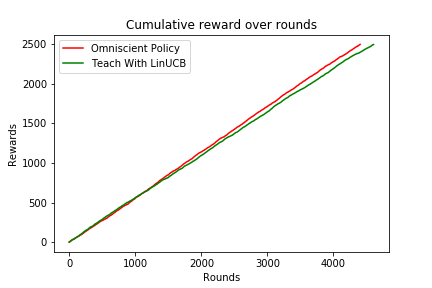
\includegraphics[scale=1.0]{Figures/cum_reward_optimal_without_confidence_threshold.png}
%     \caption{Cumulative reward without skipping.}
%     \label{cr_withoutSkip}
% \end{figure}

\begin{figure}[h]
    \centering
    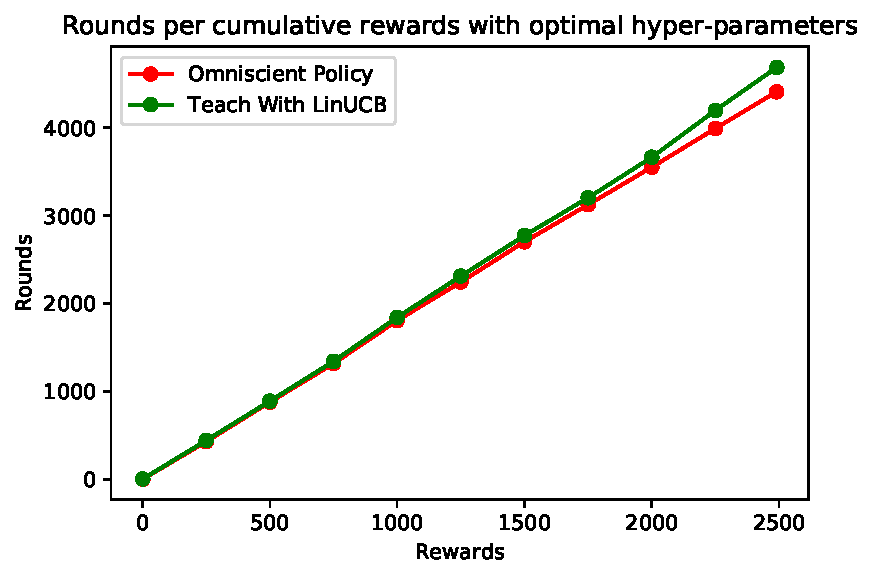
\includegraphics[scale=1.0]{Figures/rounds_per_reward_no_skipping.pdf}
    \caption{Rounds per cumulative reward without skipping.}
    \label{cr_withoutSkip}
\end{figure}

The omniscient policy required 4410 rounds to get a cumulative reward of 2490. This implies it needs 1.77 rounds for a reward (of 1). The learning algorithm required 4688 rounds to get a reward of 2491. This implies it needs 1.88 rounds for a reward (of 1). The graph (Figure \ref{chap6:rprr_no_skip}) shows the number of rounds per reward required by the algorithm at different intervals with optimal values of hyper-parameters and compares it to the omniscient policy. It shows that our learning algorithm is close to the optimal policy. \par

\begin{figure}[H]
    \centering
    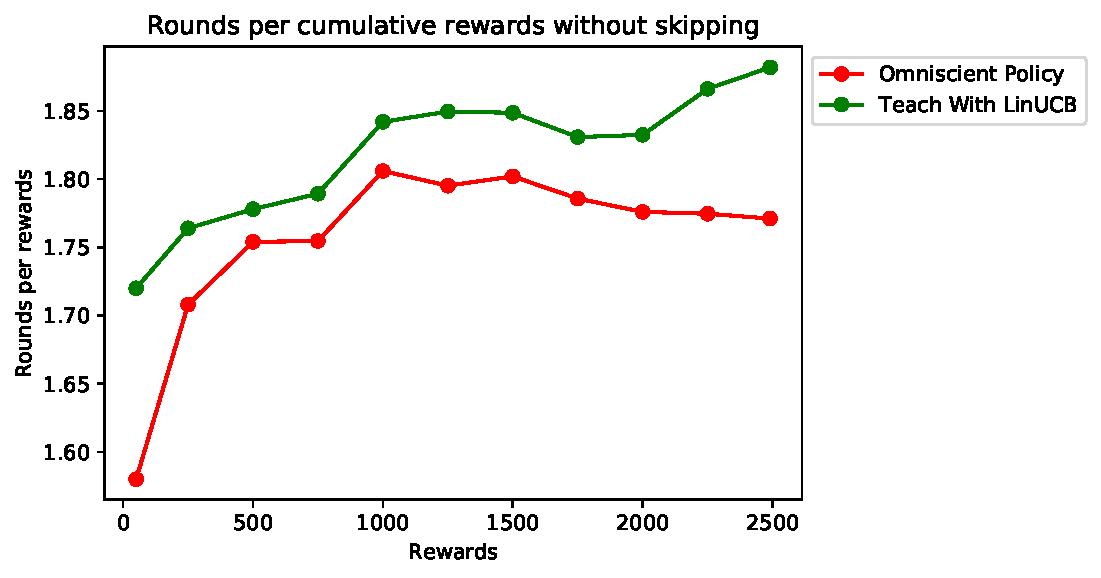
\includegraphics[scale=0.95]{Figures/rounds_per_reward_ratio_no_skipping.pdf}
    \caption{Rounds per cumulative reward ratio without skipping.}
    \label{chap6:rprr_no_skip}
\end{figure}

\subsection{With Skipping}

If a topic is not understood by a student then skipping is enabled. This does not directly imply the student would be taken to the next topic. For it to happen, the skip classifier should be confident beyond the confidence threshold to predict that it would be better to take the student to the next topic. \par 

Skipping tells the learning algorithm to skip sub-optimal content items and instead move to content items that have a higher estimated reward. This ensures that we do not present content items which are unlikely to help a student understand the topic. The graph (Figure \ref{cr_withSkip}) shows results of the learning algorithm with optimal confidence threshold $C = 30$ and $\alpha = 0.001$.

\begin{figure}[H]
    \centering
    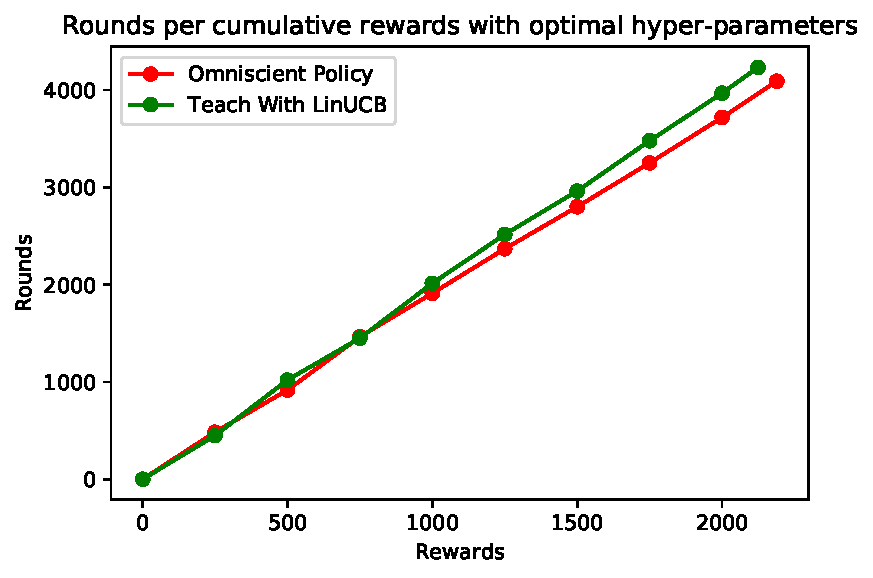
\includegraphics[scale=1.0]{Figures/rounds_per_reward_with_skipping.pdf}
    \caption{Rounds per cumulative reward with skipping}
    \label{cr_withSkip}
\end{figure}

% \begin{figure}[H]
%     \centering
%     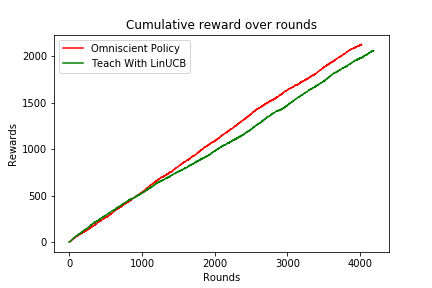
\includegraphics[scale=1.0]{Figures/cum_reward_small.png}
%     \caption{Cumulative reward with skipping}
%     \label{cr_withSkip}
% \end{figure}

The graph (Figure \ref{cr_withSkip}) shows the performance of the learning algorithm with respect to the omniscient policy. The number of rounds and the cumulative reward reduces with skipping enabled. The cumulative reward reduces as for topics that a student did not understand the skip classifier predicted with high confidence that it would be better to move to the next topic. \par

The omniscient policy required 4019 rounds to get a cumulative reward of 2128. This implies it needs 1.89 rounds for a reward (of 1). The learning algorithm required 4185 rounds to get a reward of 2062. This implies it needs 2.03 rounds for a reward (of 1). The graph (Figure \ref{chap6:rprr_skip}) shows the number of rounds per reward required by the algorithm at different intervals for optimal values of hyper-parameters and compares it to the omniscient policy. It shows that even with skipping our learning algorithm is close to the optimal policy. \par

\begin{figure}[H]
    \centering
    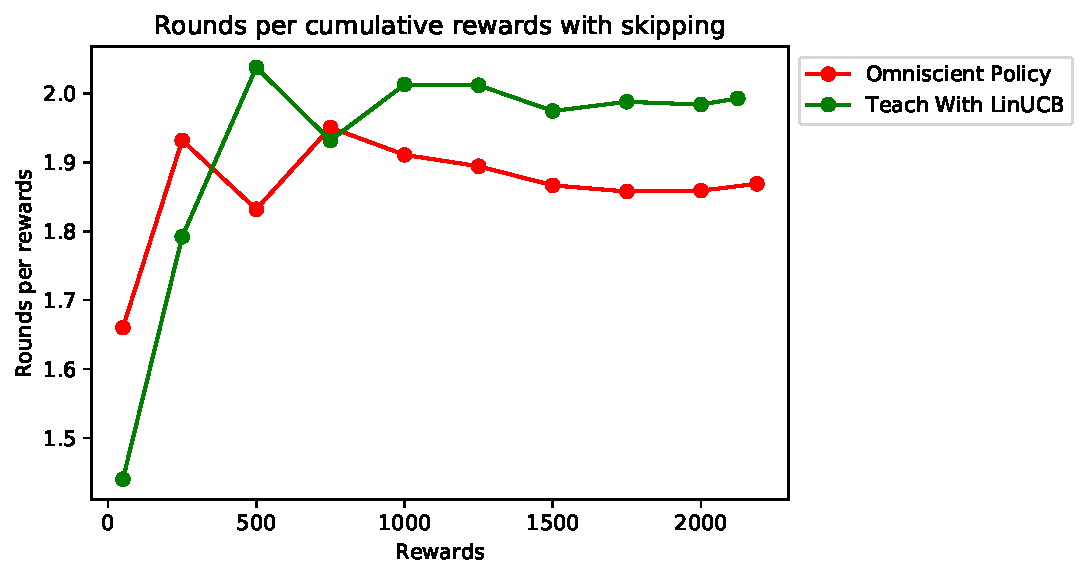
\includegraphics[scale=0.95]{Figures/rounds_per_reward_ratio_with_skipping.pdf}
    \caption{Rounds per cumulative reward ratio with skipping.}
    \label{chap6:rprr_skip}
\end{figure}

Comparing the cumulative reward graph with and without skipping shows us that our learning algorithm performs better without skipping than with skipping. However, without skipping it needs more rounds which could affect student experience. \par

% \section{Penalizing Rewards \label{chap6:pr}}

% We now update our reward assignment strategy to penalize content items which gave no rewards. This presents a different perspective as earlier in Section \ref{chap6:la} we did not penalize content items which gave no rewards. In this section rewards received by content items change from $\{0,1\}$ to $\{-1,1\}$. \par

% When content items receive no reward, the learning algorithm reduces the estimated expected reward from it. This reduces the possibility of such content items being selected which results in more content items being explored as seen in table \ref{chap6:content_items_for_alpha_with_penalty}. \par

% We follow a similar approach as before. We first find the optimal values for the hyper-parameters before we evaluate our learning algorithm. \par

% \subsection{Comparing $\alpha$}

% $\alpha$ is a scaling factor to control exploration. A higher value of $\alpha$ reduces cumulative reward as more rounds are spent exploring to find the optimal content items. The graph below shows the cumulative reward for different values of $\alpha$. 

% \begin{figure}[H]
%     \centering
%     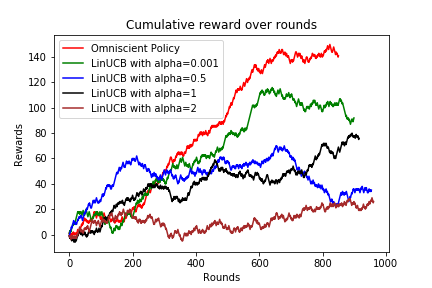
\includegraphics[scale=1.0]{Figures/penalty/cum_reward_compare_alphas.png}
%     \caption{Cumulative penalized rewards per alpha}
%     \label{cr_withSkip}
% \end{figure}

% As before $\alpha=0.001$ gives the best results compared to the omniscient policy. Below is the table which shows the number of content items explored for different values of $\alpha$. 

% \begin{table}[h]
%     \centering
%  \begin{tabular}{|c|c|}
%     \hline
%     \textrm{\textbf{Values of $\alpha$}} & \textrm{\textbf{Content Items Explored}} \\ \hline
%      \textrm{0.001} & \textrm{75}\\ \hline
%      \textrm{0.5} & \textrm{89}\\ \hline
%      \textrm{1.0} & \textrm{104}\\ \hline
%      \textrm{2.0} & \textrm{105}\\ \hline
%     \end{tabular}
%     \caption{Content items explored per $\alpha$}
%   \label{chap6:content_items_for_alpha_with_penalty}
% \end{table}

% \subsection{Confidence Threshold}

% We ran a simulation over Course 1 to find the optimal value of confidence threshold $C$. An optimal value would be one for which the skip classifier has the best performance. We ran experiments for different values of confidence threshold. The table \ref{chap6:confusion_matrix_without_ct} shows the results of the predictions made by the skip classifier with no threshold set.\par


% \begin{table}[h]
%     \centering
%     \begin{tabular}{l|l|c|c|c}
%     \multicolumn{2}{c}{}&\multicolumn{2}{c}{Predictions}&\\
%     \cline{3-4}
%     \multicolumn{2}{c|}{}&Stay (0) &Skip (1)&\multicolumn{1}{c}{Total}\\
%     \cline{2-4}
%     \multirow{2}{*}{Reward}& 0 & $74$ & $39$ & $113$\\
%     \cline{2-4}
%     & 1 & $82$ & $64$ & $146$\\
%     \cline{2-4}
%     \multicolumn{1}{c}{} & \multicolumn{1}{c}{Total} & \multicolumn{1}{c}{$156$} & \multicolumn{1}{c}{$103$} & \multicolumn{1}{c}{$518$}\\
%     \end{tabular}
%     \caption{Confusion matrix without confidence threshold}
%     \label{chap6:confusion_matrix_without_ct}
% \end{table}

% Without any threshold, our classifier would have an accuracy of 56.37 \%. The table \ref{chap6:confusion_matrix_with_ct20} shows the results for the classifier for confidence threshold of 20. This gives better results. 

% \begin{table}[h]
%     \centering
%     \begin{tabular}{l|l|c|c|c}
%     \multicolumn{2}{c}{}&\multicolumn{2}{c}{Predictions}&\\
%     \cline{3-4}
%     \multicolumn{2}{c|}{}&Stay (0) &Skip (1)&\multicolumn{1}{c}{Total}\\
%     \cline{2-4}
%     \multirow{2}{*}{Reward}& 0 & $41$ & $20$ & $61$\\
%     \cline{2-4}
%     & 1 & $59$ & $39$ & $98$\\
%     \cline{2-4}
%     \multicolumn{1}{c}{} & \multicolumn{1}{c}{Total} & \multicolumn{1}{c}{$100$} & \multicolumn{1}{c}{$59$} & \multicolumn{1}{c}{$257$}\\
%     \end{tabular}
%     \caption{Confusion matrix with confidence threshold of 20}
%     \label{chap6:confusion_matrix_with_ct20}
% \end{table}

% With a threshold set to it, our classifier would have an accuracy of 61.64\%.

% \subsection{Learning Algorithm}

% We now configure these optimal values and run a simulation of Course 2 for both the omniscient policy and the learning algorithm.  The omniscient policy knows the best arm to pull in each round. On the other hand, our learning algorithm explores to find the best content item.

% \subsubsection{No Skipping}

% We now evaluate our learning algorithm without skipping. 

% \begin{figure}[H]
%     \centering
%     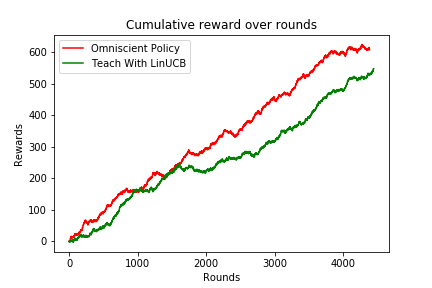
\includegraphics[scale=1.0]{Figures/penalty/cum_reward_small_NO_SKIPPING.png}
%     \caption{Cumulative penalized rewards without skipping}
%     \label{cr_withoutSkip}
% \end{figure}

% The omniscient policy took 4384 rounds compared to 4443 taken by the learning algorithm to complete the course for all students. The rewards accumulated by the omniscient policy is 608 compared to 547 by the learning algorithm. The learning algorithm performs sub-optimally, which is expected. 

% \subsubsection{With Skipping}

% With skipping enabled the ability of the learning algorithm to optimize its content item selection strategy is restricted. Skipping restricts the learning algorithm from exploring different content items to find the optimal content item in each round. The graph below shows the performance of the learning algorithm with respect to the omniscient policy with skipping enabled.

% \begin{figure}[H]
%     \centering
%     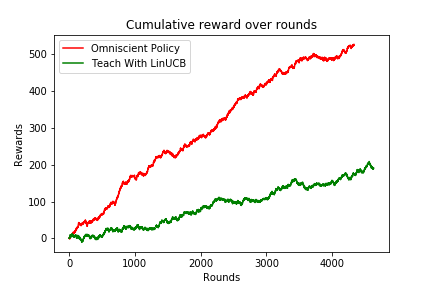
\includegraphics[scale=1.0]{Figures/penalty/cum_reward_small-WITH-SKIPPING.png}
%     \caption{Cumulative penalized rewards with skipping}
%     \label{cr_withSkip}
% \end{figure}

% The omniscient policy took 4335 rounds compared to 4634 taken by the learning algorithm to complete the course for all students. The rewards accumulated by the omniscient policy is 527 compared to 191 received by the learning algorithm. The learning algorithm performs poorly, when exploration is restricted. \par 

% With this experiment, we find that skipping although useful should only be introduced once the learning algorithm has sufficiently explored all content items. If introduced too early then skipping prevents the learning algorithm from exploring. However if introduced too late then its value diminishes. 
 
% Future Work 

% We need to come up with an approach to introduce skipping once the learning algorithm has explored sufficiently. 


% Additional optimizations 

% - Decaying confidence threshold. 
% - Pre-trained skip classifier leads to better performance. 
% - Analysis over datasets of different sizes. 